%%%%%%%%%%%%%%%%%%%%% {{{
%%Options for presentations (in-class) and handouts (e.g. print).
%\documentclass[pdf,9pt]{beamer}
\documentclass[pdf,9pt]{beamer}
% \documentclass[pdf,9pt]{beamer}


%%%%%%%%%%%%%%%%%%%%%%
%Change this for different slides so it appears in bar
\usepackage{authoraftertitle}
\date{Chapter 3. Determinants and Diagonalization \\ \S 3-2. Determinants and Matrix Inverses}

%%%%%%%%%%%%%%%%%%%%%%
%% Upload common style file
\usepackage{LyryxLAWASlidesStyle}

\begin{document}

%%%%%%%%%%%%%%%%%%%%%%%
%% Title Page and Copyright Common to All Slides

%Title Page
\input frontmatter/titlepage.tex

%LOTS Page
\input frontmatter/lyryxopentexts.tex

%Copyright Page
\input frontmatter/copyright.tex

%%%%%%%%%%%%%%%%%%%%%%%%% }}}
%-------------- start slide -------------------------------%{{{ 2
\begin{frame}[fragile]
   \tableofcontents
\end{frame}
%-------------- end slide -------------------------------%}}}
\section[\textcolor{yellow}{}]{\textcolor{yellow}{Determinants and Matrix Inverses}}
%-------------- start slide -------------------------------%{{{ 3
\frame{
\frametitle{Determinants and Matrix Inverses}
\pause
\begin{theorem}[Product Theorem]
    If $A$ and $B$ are $n\times n$ matrices, then
    \[ \det(AB)=\det A \det B.\]
\end{theorem}
\vfill
\pause
\begin{proof}
\small
    If either $A$ or $B$ is singular, then both sides are equal to zero.
    \bigskip
    \pause

    Now assume that both $A$ and $B$ are nonsingular, i.e., $\rank(A)=\rank(B)=n$.
    Then
    \begin{align*}
        \text{rref}(A) = \text{rref}(B) = I
    \end{align*}
    \pause
    and
    \begin{align*}
        A = E_1E_2\cdots E_{p} \quad\text{and}\quad
        B = F_1F_2\cdots F_{q}.
    \end{align*}
    where $E_i$ and $F_j$ are elementary matrices. \pause Then by the relation of elementary row operations with determinants (Theorem 3.1.2), we see that
\begin{align*}
    |AB| & = |E_1\cdots E_p F_1\cdots F_q| \\
         & = |E_1|\cdots |E_p| |F_1|\cdots |F_q|\\
         & = |E_1\cdots E_p| |F_1\cdots F_q|\\
         & = |A| |B|.
\end{align*}
\end{proof}
}
%-------------- end slide -------------------------------%}}}
%-------------- start slide -------------------------------%{{{ 3
\frame{
\begin{theorem}[Determinant of Matrix Inverse]
    An $n\times n$ matrix $A$ is invertible if and only if
    \alert{$\det A\neq 0$}.
    In this case,
    \[ \det(A^{-1})=\left(\det A\right)^{-1} = \frac{1}{\det A}.\]
\end{theorem}
\pause
\vfill
\begin{proof}
    \small
    "$\Rightarrow$":
   \begin{align*}
       1 = |I| = |A A^{-1}| = |A| |A^{-1}|
       \quad\Rightarrow\quad
       \begin{cases}
            |A| \ne 0 \\[ 1em ]
            |A^{-1}| = \frac{1}{|A|}.
       \end{cases}
   \end{align*}
  \pause

  "$\Leftarrow$": If $|A|\ne 0$, then $\text{rref}(A)=I$ because otherwise one obtains contradiction by Theorem 3.1.2. This is another way to say that $A$ is invertible: (recall the matrix inverse algorithm)
  \begin{align*}
      \left[A|I\right] \to \bigg[\underbrace{\text{rref}(A)}_{\displaystyle =I}\bigg| A^{-1}\bigg].
  \end{align*}
\end{proof}
}
%-------------- end slide -------------------------------%}}}
%-------------- start slide -------------------------------%{{{ 4
\frame{
\begin{example}
Find all values of $c$ for which
$A=\left[\begin{array}{rrr}
    c  & 1 & 0 \\
    0  & 2 & c \\
    -1 & c & 5
\end{array}\right]$ is invertible.

\uncover<2->{
\[
\det A = \left|\begin{array}{rrr}
    c  & 1 & 0 \\
    0  & 2 & c \\
    -1 & c & 5
\end{array}\right| =
c  \left|\begin{array}{rr}
 2 & c \\
 c & 5
\end{array}\right| +
(-1) \left|\begin{array}{rr}
 1 & 0 \\
 2 & c
\end{array}\right|\]
}
\uncover<3->{
\[ =c(10-c^2)-c = c(9-c^2)=c(3-c)(3+c).\]}
\medskip

\uncover<4->{
Therefore, $A$ is invertible for all $c\neq 0, 3, -3$.
}
\end{example}
}
%-------------- end slide -------------------------------%}}}
%-------------- start slide -------------------------------%{{{ 5
\frame{
\begin{theorem}[Determinant of Matrix Transpose]
If $A$ is an $n\times n$ matrix, then $\det(A^T)=\det A$.
\end{theorem}
\vfill
\pause
\begin{proofnoend}
    \begin{enumerate}
      \item This is trivially true for all elementary matrices.
      \pause
      \item If $A$ is not invertible, then neither is $A^T$. Hence, $\det A = 0 = \det A^T$.
      \pause
      \item If $A$ is invertible, then $A= E_k E_{k-1} \cdots E_2E_1$. Hence, by Case 1,
          \begin{align*}
              \left|A^T\right| & = \left|\left(E_k E_{k-1} \cdots E_2E_1\right)^T\right|                                     \\
                               & = \left|E_1^T E_2^T \cdots E_{k-1}^TE_k^T\right|                                            \\
                               & = \left|E_1^T\right| \left| E_2^T \right| \cdots  \left|E_{k-1}^T\right| \left|E_k^T\right| \\
                               & = \left|E_1\right| \left| E_2 \right| \cdots \left|E_{k-1}\right| \left|E_k\right|          \\
                               & = \left|E_k\right| \left| E_{k-1} \right| \cdots \left|E_2\right| \left|E_1\right|          \\
                               & = \left|E_k E_{k-1} \cdots E_2 E_1\right|                                                   \\
                               & = \left|A\right|.
          \end{align*}
    \end{enumerate}
    \myQED
\end{proofnoend}
}
%-------------- end slide -------------------------------%}}}
%-------------- start slide -------------------------------%{{{ 6
\frame{
\begin{problem}
Suppose $A$ is a $3\times 3$ matrix.
Find $\det A$ and $\det B$ if
\[ \det(2A^{-1})=-4=\det(A^3(B^{-1})^T).\]
\end{problem}
\pause
\vfill
\begin{solution}
First,
    \begin{eqnarray*}
\det(2A^{-1}) & = & -4 \\
    2^3\det(A^{-1}) & = & -4 \\
    \frac{1}{\det A} & = & \frac{-4}{8} = -\frac{1}{2}
\end{eqnarray*}
\uncover<3->{
Therefore, $\det A=-2$.}
\end{solution}
}
%-------------- end slide -------------------------------%}}}
%-------------- start slide -------------------------------%{{{ 7
\frame{
\begin{solution}[continued]
Now,
\begin{eqnarray*}
\det(A^{3}(B^{-1})^T) & = & -4 \\
(\det A)^3\det(B^{-1}) & = & -4 \\
(-2)^3\det(B^{-1}) & = & -4 \\
(-8)\det(B^{-1}) & = & -4 \\
\frac{1}{\det B} & = & \frac{-4}{-8} = \frac{1}{2}
\end{eqnarray*}
\pause
Therefore, $\det B=2$.\myQED
\end{solution}
}
%-------------- end slide -------------------------------%}}}
%-------------- start slide -------------------------------%{{{ 8
\frame{
\begin{problem}
Suppose $A$, $B$ and $C$ are $4\times 4$ matrices with
\[ \det A = -1, \det B = 2, \quad\text{and}\quad \det C=1.\]
Find $\det(2A^2(B^{-1})(C^T)^3 B(A^{-1}))$.
\end{problem}
\vfill
\pause
\begin{solution}
    \begin{eqnarray*}
        \det(2A^2(B^{-1})(C^T)^3 B(A^{-1}))
            & = & 2^4 (\det A)^2 \frac{1}{\det B}(\det C)^3 (\det B)\frac{1}{\det A} \\
            & = & 16(\det A)(\det C)^3                                               \\
            & = & 16\times (-1)\times 1^3                                            \\
            & = & -16.
    \end{eqnarray*}
    \myQED
\end{solution}
}
%-------------- end slide -------------------------------%}}}
%-------------- start slide -------------------------------%{{{ 9
\frame{
\begin{problem}
A square matrix $A$ is \alert{orthogonal} if and only if
$A^T=A^{-1}$.
What are the possible values of $\det A$ if $A$ is orthogonal?
\end{problem}
\vfill
\pause
\begin{solution}
    Since $A^T=A^{-1}$,
    \begin{eqnarray*}
        \det A^T   & = & \det(A^{-1})     \\
        \det A     & = & \frac{1}{\det A} \\
        (\det A)^2 & = & 1
    \end{eqnarray*}
    \pause
    Assuming $A$ is a \alert{real} matrix, this implies that
    $\det A = \pm 1$, i.e., $\det A=1$ or $\det A = -1$.
    \myQED
\end{solution}
}
%-------------- end slide -------------------------------%}}}
\section[\textcolor{yellow}{}]{\textcolor{yellow}{Adjugates}}
%-------------- start slide -------------------------------%{{{ 10
\frame{
\frametitle{Adjugates}
\pause
\begin{emptytitle}
    For a $2\times 2$ matrix
    $A=\left[\begin{array}{cc} a & b \\ c & d \end{array}\right]$,
    we have already seen the \alert{adjugate} of $A$ defined as
    \[ \adj (A) =
	\left[\begin{array}{cc}
	    d  & -b \\
	    -c & a
	\end{array}\right],
    \]
    and observed that
    \begin{eqnarray*}
      A\:\adj(A) & = & \left[\begin{array}{cc} a     & b \\ c & d \end{array}\right] \left[\begin{array}{cc} d  & -b \\ -c & a \end{array}\right] \\
                 & = & \left[\begin{array}{cc} ad-bc & 0 \\ 0 & ad-bc \end{array}\right]                       \\
                 & = & (\det A) I_2
    \end{eqnarray*}
    \pause
    Furthermore, if $\det A\neq 0$, then $A$ is invertible and
    \[ A^{-1} = \frac{1}{\det A} \adj(A).\]
\end{emptytitle}
}
%-------------- end slide -------------------------------%}}}
%-------------- start slide -------------------------------%{{{ 11
\frame{
\begin{definition}[Adjugate Matrix]
    If $A$ is an $n\times n$ matrix, then the \textcolor{yellow}{adjugate matrix of $A$} is defined to be
    \[
        \adj(A) \stackrel{\text{def}}{=} \left[\begin{array}{c} c_{ij}(A) \end{array}\right]^T= \left[\begin{array}{c} (-1)^{i+j} \det(A_{ij}) \end{array}\right]^T,
    \]
    where $c_{ij}(A)$ is the $(i,j)$-cofactor of $A$,
    i.e., $\adj(A)$ is the transpose of the
    \alert{cofactor matrix} (matrix of cofactors).
\end{definition}
}
%-------------- end slide -------------------------------%}}}
%-------------- start slide -------------------------------%{{{ 12
\frame{
\begin{problem}
    Find $\adj(A)$ when
    $A=\left[\begin{array}{rrr}
        2 & 1  & 3 \\
        5 & -7 & 1 \\
        3 & 0  & -6
    \end{array}\right]$ and compute $A\:\adj(A)$.
\end{problem}
\pause
\vfill
\begin{solution}
\[
    \adj(A) =
    \left[\begin{array}{rrr}
    42 & 6 & 22 \\
        33 & -21 & 13 \\
        21 & 3 & -19
        \end{array}\right].
\]
\pause
Notice that
\begin{eqnarray*}
    A\: \adj(A) & = & \left[\begin{array}{rrr}
            2 & 1  & 3 \\
            5 & -7 & 1 \\
            3 & 0  & -6
        \end{array}\right]
        \left[\begin{array}{rrr}
            42 & 6   & 22 \\
            33 & -21 & 13 \\
            21 & 3   & -19
        \end{array}\right]
         =
        \left[\begin{array}{ccc}
            180 & 0   & 0 \\
            0   & 180 & 0 \\
            0   & 0   & 180
        \end{array}\right]
\end{eqnarray*}
\pause
\begin{eqnarray*}
    \det A  =
    \left|\begin{array}{rrr}
        2 & 1  & 3 \\
        5 & -7 & 1 \\
        3 & 0  & -6
    \end{array}\right|
     =
    \left|\begin{array}{rrr}
        2  & 1 & 3  \\
        19 & 0 & 22 \\
        3  & 0 & -6
    \end{array}\right|
     =
    (-1)\left|\begin{array}{rrr}
        19 & 22 \\
        3  & -6
    \end{array}\right|
     =  180,
    \end{eqnarray*}
    \pause
    Therefore,\[ A\: \adj(A)=(\det A) I.\]
    \myQED
\end{solution}
}
%-------------- end slide -------------------------------%}}}
% %-------------- start slide -------------------------------%{{{ 13 -- removed.
% \frame{
% \begin{solution}[continued]
%     Also,
%     \begin{eqnarray*}
%     \det A & = &
%     \left|\begin{array}{rrr}
%         2 & 1  & 3 \\
%         5 & -7 & 1 \\
%         3 & 0  & -6
%     \end{array}\right| \\
%     & = &
%     \left|\begin{array}{rrr}
%         2  & 1 & 3  \\
%         19 & 0 & 22 \\
%         3  & 0 & -6
%     \end{array}\right| \\
%     & = &
%     (-1)\left|\begin{array}{rrr}
%         19 & 22 \\
%         3  & -6
%     \end{array}\right| \\
%     & = & 180,
%     \end{eqnarray*}
%
%     \pause
%     so \alert{in this example}, we see that
%         \[ A\: \adj(A)=(\det A) I.\]
%     \myQED
% \end{solution}
% }
% %-------------- end slide -------------------------------%}}}
%-------------- start slide -------------------------------%{{{ 14
\frame{
\begin{theorem}[The Adjugate Formula]
    If $A$ is an $n\times n$ matrix, then
    \[ A\: \adj(A) = (\det A)I =\: \adj(A) A.\]
    Furthermore, \alert{if $\det A\neq 0$}, then
    \[ A^{-1} = \frac{1}{\det A} \adj(A).\]
\end{theorem}
\bigskip
\vfill
\begin{proof}
\small
    We only prove the case when $n=3$.
% \begin{equation*}
% \adj(A) = \leftB \begin{array}{rrr}
%   c_{11} & c_{12} & c_{13} \\
%   c_{21} & c_{22} & c_{23} \\
%   c_{31} & c_{32} & c_{33}
% \end{array}\rightB^T = \leftB \begin{array}{rrr}
%   c_{11} & c_{21} & c_{31} \\
%   c_{12} & c_{22} & c_{32} \\
%   c_{13} & c_{23} & c_{33}
% \end{array}\rightB
% \end{equation*}
% If $A = \leftB a_{ij} \rightB$ in the usual notation, we are to verify that $A(\func{adj }A) = (\func{det }A)I$. That is,
\begin{equation*}
A\: \adj(A) =\leftB \begin{array}{rrr}
  a_{11} & a_{12} & a_{13} \\
  a_{21} & a_{22} & a_{23} \\
  a_{31} & a_{32} & a_{33}
\end{array}\rightB \leftB \begin{array}{rrr}
  c_{11} & c_{21} & c_{31} \\
  c_{12} & c_{22} & c_{32} \\
  c_{13} & c_{23} & c_{33}
\end{array}\rightB
 = \leftB \begin{array}{ccc}
  |A| & 0                     & 0 \\
  0   & |A|                   & 0 \\
  0   & \textcolor{red}{0} & |A|
\end{array}\rightB
\end{equation*}
where, for example,
\begin{align*}
   \textcolor{red}{\small\text{(3,2)-th entry}}
   & = \textcolor{yellow}{a_{31}}c_{21} + \textcolor{yellow}{a_{32}}c_{22}+\textcolor{yellow}{a_{33}}c_{23} \\
   & = \det \begin{bmatrix}
       a_{11} & a_{12} & a_{13}\\
       a_{31} & a_{32} & a_{33}\\
       a_{31} & a_{32} & a_{33}\\
   \end{bmatrix}
   =
   \textcolor{red}{0}.
\end{align*}
\end{proof}
}
%-------------- end slide -------------------------------%}}}
%-------------- start slide -------------------------------%{{{ 15
\frame{
\begin{example}
For an $n\times n$ matrix $A$, show that
$\det\: \adj(A)=(\det A)^{n-1}$.

\bigskip
\uncover<2->{
Using the adjugate formula,
\begin{eqnarray*}
A\: \adj(A) & = & (\det A)I \\
\det(A\: \adj(A)) & = & \det((\det A)I) \\
(\det A) \times \det\: \adj(A) & = & (\det A)^{n}(\det I) \\
(\det A) \times \det\: \adj(A) & = & (\det A)^{n}
\end{eqnarray*}}
\uncover<3->{
If $\det A\neq 0$, then divide both sides of the last equation
by $\det A$:
\[ \det\: \adj(A)=(\det A)^{n-1}.\]}
\end{example}
}
%-------------- end slide -------------------------------%}}}
%-------------- start slide -------------------------------%{{{ 16
\frame{
\begin{example}[continued]
For the case $\det A=0$, we claim that
\begin{align}
    \tag{\star}
    \det A = 0 \quad \Rightarrow \quad
    \det\: \adj(A) =0,
\end{align}
\pause
which implies that
\[ \det \: \adj(A)=0= 0^{n-1}=(\det A)^{n-1}.\]
\end{example}
\vfill
\pause

\begin{proofnoend}[of (\star)]
    We will prove (\star) by contradiction. \pause
    Indeed, if $\det A=0$, then
    \[ A\: \adj(A) = (\det A)I = (0)I=O,\]
    i.e., $A\: \adj(A)$ is the zero matrix.
    \pause
    If $\alert{\det \: \adj(A)\ne 0}$,
    then $\adj(A)$ would
    be invertible, and $A\: \adj(A) = O$ would imply $A=O$. \pause
    However, if $A=O$, then $\adj(A)=O$ and is {\bf not} invertible,
    and thus has determinant equal to zero, i.e.,
    $\alert{\det \: \adj(A)= 0}$, (a contradiction!)
    \pause
    Therefore, $\alert{\det \: \adj(A)= 0}$, i.e., (\star) is true.
    \myQED
\end{proofnoend}
}
%-------------- end slide -------------------------------%}}}
%-------------- start slide -------------------------------%{{{ 17
\frame{
\begin{problem}
Let $A$ and $B$ be $n\times n$ matrices.
Show that $\det(A+B^T)=\det(A^T+B)$.
\end{problem}
\pause
\vfill
\begin{solution}
Notice that
\[ (A+B^T)^T = A^T + (B^T)^T = A^T + B.\]

Since a matrix and it's transpose have the same determinant
\begin{eqnarray*}
\det(A+B^T) = \det((A+B^T)^T)  =  \det(A^T + B).
\end{eqnarray*}
\myQED
\end{solution}
%\vspace*{2in}
}
%-------------- end slide -------------------------------%}}}
%-------------- start slide -------------------------------%{{{ 18
\frame{
\begin{problem}
    For each of the following statements, determine if it is true
    or false, and supply a proof or a counterexample.
    \begin{enumerate}
        \item If $\adj(A)$ exists, then $A$ is invertible.
        \item If $A$ and $B$ are $n\times n$ matrices, then $\det (AB)=\det (B^TA)$.
    \end{enumerate}
\end{problem}
\vfill
\pause
\begin{problem}
    Prove or give a counterexample to the following statement:
    \begin{center}
    If $\det A=1$, then $\adj(A)=A$.
    \end{center}
\end{problem}
}
%-------------- end slide -------------------------------%}}}
\section[\textcolor{yellow}{}]{\textcolor{yellow}{Cramer's Rule}}
%-------------- start slide -------------------------------%{{{ 19
\frame{
\frametitle{Cramer's Rule}
\pause
\begin{emptytitle}
    If $A$ is an $n\times n$ \alert{invertible} matrix, then
    the solution to $A\vec{x}=\vec{b}$ can be given in terms of determinants
    of matrices.
\end{emptytitle}
\vfill
\pause
\begin{theorem}[Cramer's Rule]
    Let $A$ be an $n\times n$ invertible matrix, the
    solution to the system $A\vec{x}=\vec{b}$ of $n$ equations in teh variables
    $x_1$, $x_2 \cdots  x_n$ is given by
    \[
	x_1 = \frac{\det\left( A_1(\vec{b}) \right)}{\det A},\quad
	x_2 = \frac{\det\left( A_2(\vec{b}) \right)}{\det A},\quad \cdots, \quad
	x_n = \frac{\det\left( A_n(\vec{b}) \right)}{\det A}
    \]
    where, for each $j$, the matrix $A_j(\vec{b})$ is obtained from $A$ by
    replacing column $j$ with $\vec{b}$:
    \begin{align*}
    A_j(\vec{b}) = \left[ \begin{array}{ccccccc} \vec{a}_1 & \cdots & \vec{a}_{j-1} & \vec{b} & \vec{a}_{j+1} & \cdots & \vec{a}_n \end{array} \right]
    \end{align*}
\end{theorem}
}
%-------------- end slide -------------------------------%}}}
%-------------- start slide -------------------------------%{{{ 20
\begin{frame}[fragile]
\begin{proofnoend}
    \begin{itemize}
        \item
	Notice that
	\begin{eqnarray*}
	A_j(\vec{b}) & = & \left[ \begin{array}{ccccccc} \; \vec{a}_1 & \;\, \cdots & \; \vec{a}_{j-1} & \;\,\vec{b} & \;\;\, \vec{a}_{j+1} & \;\, \cdots & \;\vec{a}_n  \;\,\, \end{array} \right] \\
	& = &  \left[ \begin{array}{ccccccc} A\vec{e}_1 & \cdots & A\vec{e}_{j-1} & A\vec{x} & A\vec{e}_{j+1} & \cdots & A\vec{e}_n \end{array} \right] \\
	& = & \!\!\!\!\! A  \left[ \begin{array}{ccccccc} \; \vec{e}_1 & \;\, \cdots & \; \vec{e}_{j-1} & \;\,\vec{x} & \;\;\, \vec{e}_{j+1} & \;\, \cdots & \;\vec{e}_n  \;\,\, \end{array} \right] \\
	& & \\
	& = & \!\!\!\!\! A \; I_j(\vec{x})
	\end{eqnarray*}
    \pause
    \vspace{-1em}
    \item[] where
    \begin{align*}
	I_j(\vec{x}) &= \left[ \begin{array}{ccccccc}
	\vec{e}_1 & \cdots & \vec{e}_{j-1} & \vec{x} & \vec{e}_{j+1} & \cdots & \vec{e}_n \end{array} \right] \\
	&
	=
	\left[ \begin{array}{ccccccc}
	1 &  & & x_1 & & & \\ & \ddots & & \vdots & & & \\ & & 1 & x_{j-1} & & & \\
	& & & x_{j} & & & \\ & & & x_{j+1} & 1 & & \\ & & & \vdots & & \ddots & \\ & & & x_n & & & 1
	\end{array} \right]
    \end{align*}
    \end{itemize}
\end{proofnoend}
\end{frame}
%-------------- end slide -------------------------------%}}}
%-------------- start slide -------------------------------%{{{ 21
\begin{frame}[fragile]
    \begin{proofnoend}[continued]
    \begin{itemize}
	\item Hence, by taking the determinants on both sides, we have
	\begin{eqnarray*}
	\det(A_j(\vec{b})) & = & \det(A \; I_j(\vec{x})) \\
	& = & \det(A)\det(I_j(\vec{x}))
	\end{eqnarray*}
	\item
	And because $\det(A) \neq 0$, we can then write:
	$$
	\det(I_j(\vec{x})) = \frac{\det(A_j(\vec{b}))}{\det(A)}
	$$
	\item
	Finally, notice that $\qquad \det(I_j(\vec{x}))=\cdots $ \pause $ = x_j$.
    \end{itemize}
    \myQED
\end{proofnoend}
\end{frame}
%-------------- end slide -------------------------------%}}}
%-------------- start slide -------------------------------%{{{ 22
\frame{
\begin{problem}
Find $x_3$ such that
\[ \begin{array}{rrrrrrr}
3x_1 & + & x_2 & - & x_3 & = & -1 \\
5x_1 & + & 2x_2 & & & = & 2 \\
x_1 & + & x_2 & - & x_3 & = & 1
\end{array}\]
\end{problem}
\vfill
\pause
\begin{solution}
    By Cramer's rule, $x_3=\frac{\det A_3}{\det A}$, where
    \[ A=\left[\begin{array}{rrr}
            3 & 1 & -1 \\
            5 & 2 & 0 \\
            1 & 1 & -1
        \end{array}\right]
        \quad\text{and}\quad
        A_3=\left[\begin{array}{rrr}
            3 & 1 & -1 \\
            5 & 2 & 2 \\
            1 & 1 & 1
        \end{array}\right].
     \]
   \pause
    Computing the determinants of these two matrices,
    \[ \det A = -4 \quad\text{and}\quad \det A_3 = -6.\]
    \pause
    Therefore, $x_3=\frac{-6}{-4}=\frac{3}{2}$.
    \myQED
\end{solution}
}
%-------------- end slide -------------------------------%}}}
%-------------- start slide -------------------------------%{{{ 23
\frame{
\begin{remark}
For practice, you should compute $\det A_1$ and $\det A_2$,
where
\[ A_1=\left[\begin{array}{rrr}
    -1 & 1 & -1 \\
    2  & 2 & 0  \\
    1  & 1 & -1
\end{array}\right]
\quad\text{and}\quad
A_2=\left[\begin{array}{rrr}
    3 & -1 & -1 \\
    5 & 2  & 0  \\
    1 & 1  & -1
\end{array}\right],\]
and then solve for $x_1$ and $x_2$.
\bigskip

\pause
{\bf Solution.} $x_1=-1$, $x_2=7/2$. \myQED
\end{remark}
}

%-------------- end slide -------------------------------%}}}
\section[\textcolor{yellow}{}]{\textcolor{yellow}{Polynomial Interpolation and Vandermonde Determinant}}
%-------------- start slide -------------------------------%{{{ 24
\frame{
\frametitle{Polynomial Interpolation and Vandermonde Determinant}
\pause
\begin{problem}
    Given data points $(0,1)$, $(1,2)$, $(2,5)$ and $(3,10)$,
    find an interpolating polynomial
    $p(x)$ of degree at most three,
    and then estimate the value of $y$ corresponding to $x=3/2$.
\end{problem}
\vfill
\begin{center}
    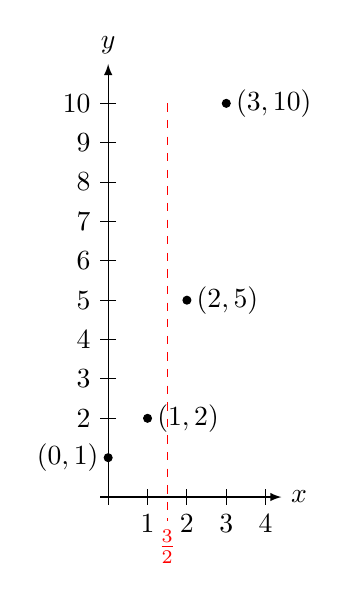
\begin{tikzpicture}[scale=1, transform shape]
    \tikzset{>=latex}
    \draw [->] (-0.1,0) -- (2.2,0) node [right] {$x$};
    \draw [->] (0,-0.1) -- (0,5.5)  node [above] {$y$};

    \coordinate (1) at (0,0.5);
    \coordinate (2) at (0.5,1);
    \coordinate (3) at (1,2.5);
    \coordinate (4) at (1.5,5);

    \node at (1) [left] {$(0,1)$};
    \node at (2) [right] {$(1,2)$};
    \node at (3) [right] {$(2,5)$};
    \node at (4) [right] {$(3,10)$};

    \foreach \x in {1,2,3,4}{
	\draw (\x/2,0.1) -- (\x/2,-0.1) node [below] {$\x$};
    }
    \foreach \y in {2,3,4,5,6,7,8,9,10}{
	\draw (0.1,\y/2) -- (-0.1,\y/2) node [left] {$\y$};
    }
    \foreach \x in {1,2,3,4}{
	\filldraw (\x) circle (0.05);
    }
    \pause
    \draw [dashed,color=red] (3/4,5) -- (3/4,-0.3) node [below] {$\frac{3}{2}$};
    \end{tikzpicture}
\end{center}
}
%-------------- end slide -------------------------------%}}}
%-------------- start slide -------------------------------%{{{ 25
\begin{frame}[fragile]
\begin{solution}
We want to find the coefficients $r_0$, $r_1$, $r_2$ and $r_3$ of
\[ p(x) = r_0 + r_1 x + r_2 x^2 + r_3 x^3\]
so that $p(0)=1$, $p(1)=2$, $p(2)=5$, and $p(3)=10$.
\begin{eqnarray*}
p(0) & = & r_0 = 1\\
p(1) & = & r_0 + r_1 + r_2 + r_3 = 2 \\
p(2) & = & r_0 + 2r_1 + 4r_2 + 8r_3 = 5 \\
p(3) & = & r_0 + 3r_1 + 9r_2 + 27r_3 = 10
\end{eqnarray*}
\end{solution}
\end{frame}
%-------------- end slide -------------------------------%}}}
%-------------- start slide -------------------------------%{{{ 26
\frame{
\begin{solution}[continued]
Solve this system of four equations in the four variables
$r_0$, $r_1$, $r_2$ and $r_3$.
\pause
\[
    \left[\begin{array}{rrrr|r}
        1 & 0 & 0 & 0  & 1 \\
        1 & 1 & 1 & 1  & 2 \\
        1 & 2 & 4 & 8  & 5 \\
        1 & 3 & 9 & 27 & 10
    \end{array}\right]
    \rightarrow \cdots \rightarrow
    \left[\begin{array}{rrrr|r}
        1 & 0 & 0 & 0 & 1 \\
        0 & 1 & 0 & 0 & 0 \\
        0 & 0 & 1 & 0 & 1 \\
        0 & 0 & 0 & 1 & 0
    \end{array}\right]
\]

\pause
Therefore, $r_0=1$, $r_1=0$, $r_2=1$, $r_3=0$, and so
    \[ p(x)= 1 + x^2.\]
\pause
Finally, the estimate is
\[
    y=p\left(\frac{3}{2}\right) = 1 + \left(\frac{3}{2}\right)^2=\frac{13}{4}.
\]
\myQED
\end{solution}
}
%-------------- end slide -------------------------------%}}}
%-------------- start slide -------------------------------%{{{ 27
\begin{frame}[fragile]
\begin{center}
    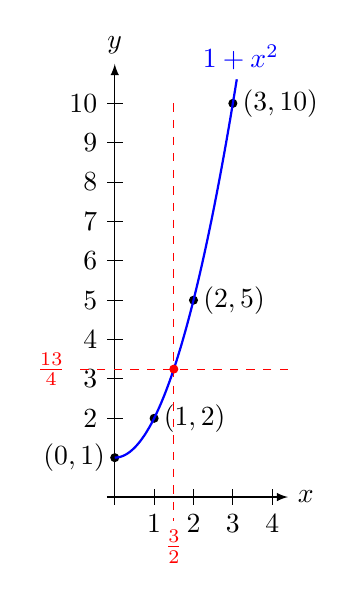
\begin{tikzpicture}[scale=1, transform shape]
    \tikzset{>=latex}
    \draw [->] (-0.1,0) -- (2.2,0) node [right] {$x$};
    \draw [->] (0,-0.1) -- (0,5.5)  node [above] {$y$};

    \coordinate (1) at (0,0.5);
    \coordinate (2) at (0.5,1);
    \coordinate (3) at (1,2.5);
    \coordinate (4) at (1.5,5);

    \node at (1) [left] {$(0,1)$};
    \node at (2) [right] {$(1,2)$};
    \node at (3) [right] {$(2,5)$};
    \node at (4) [right] {$(3,10)$};

    \foreach \x in {1,2,3,4}{
	\draw (\x/2,0.1) -- (\x/2,-0.1) node [below] {$\x$};
    }
    \foreach \y in {2,3,4,5,6,7,8,9,10}{
	\draw (0.1,\y/2) -- (-0.1,\y/2) node [left] {$\y$};
    }
    \foreach \x in {1,2,3,4}{
	\filldraw (\x) circle (0.05);
    }
    \draw [dashed,color=red] (3/4,5) -- (3/4,-0.3) node [below] {$\frac{3}{2}$};
    \draw [dashed,color=red] (2.2,13/8) -- (-0.5,13/8) node [left] {$\frac{13}{4}$};
    \draw[scale=0.5, domain=0:3.1, smooth, thick, variable=\x, blue] plot ({\x}, {1+\x*\x});
    \node at (1.6,5.3) [above,color=blue] {$1+x^2$};
    \filldraw [color=red] (3/4,13/8) circle (0.05);

    % \coordinate (Q) at (3,0.3);
    % \coordinate (0) at (0,0);
    % \draw (P) -- coordinate[pos={1/3}] (A) coordinate[pos={2/3}] (B) (Q) node [right] {$Q$};
    % \draw [->,dashed] (0) node [below] {$P$} -- (P) node [above] {$P$};
    % \draw [->,dashed] (0) -- (A) node [above] {$A$};
    % \draw [->,dashed] (0) -- (B) node [above] {$B$};
    % \filldraw (P) circle (0.05);
    % \filldraw (Q) circle (0.05);
    % \filldraw (0) circle (0.05);
    % \filldraw (A) circle (0.05);
    % \filldraw (B) circle (0.05);
    \end{tikzpicture}
\end{center}
\end{frame}
%-------------- end slide -------------------------------%}}}
%-------------- start slide -------------------------------%{{{ 28
\frame{
\begin{theorem}[Polynomial Interpolation]
    Given $n$ data points $(x_1,y_1), (x_2,y_2),\ldots ,
    (x_n,y_n)$ with the $x_i$ \alert{distinct}, there is a
    unique polynomial
    \[ p(x)= r_0 + r_1x + r_2x^2 +\cdots + r_{n-1}x^{n-1}\]
    such that $p(x_i)=y_i$ for $i=1,2,\ldots,n$.
\end{theorem}
\vfill
\pause
\begin{emptytitle}
    The polynomial $p(x)$ is called the \alert{interpolating polynomial}
    for the data.
\end{emptytitle}
}
%-------------- end slide -------------------------------%}}}
%-------------- start slide -------------------------------%{{{ 29
\frame{
\begin{emptytitle}
    To find $p(x)= r_0 + r_1x + r_2x^2 +\cdots + r_{n-1}x^{n-1}$, set up a system of $n$ linear equations in the $n$
    variables $r_0, r_1, r_2, \ldots, r_{n-1}$.
\[ \begin{array}{ccc}
    r_0 + r_1x_1 + r_2x_1^2 + \cdots + r_{n-1}x_1^{n-1} & = & y_1 \\[0.5em]
    r_0 + r_1x_2 + r_2x_2^2 + \cdots + r_{n-1}x_2^{n-1} & = & y_2 \\[0.5em]
    r_0 + r_1x_3 + r_2x_3^2 + \cdots + r_{n-1}x_3^{n-1} & = & y_3 \\[0.5em]
    \vdots & \vdots & \vdots \\[0.5em]
    r_0 + r_1x_n + r_2x_n^2 + \cdots + r_{n-1}x_n^{n-1} & = & y_n
\end{array} \]
\pause
The coefficient matrix for this system is
\bigskip
\[
    \textcolor{yellow}{\left[\begin{array}{ccccc}
        1      & x_1    & x_1^2  & \cdots & x_1^{n-1}\\
        1      & x_2    & x_2^2  & \cdots & x_2^{n-1}\\
        \vdots & \vdots & \vdots & \vdots & \vdots \\
        1      & x_n    & x_n^2  & \cdots & x_n^{n-1}
    \end{array}\right]}
\]
\pause
\bigskip
\begin{itemize}
    \item Such matrix is called \textcolor{yellow}{Vandermonde matrix}.
    \item Its determinant is called \textcolor{yellow}{Vandermonde determinant}.
\end{itemize}
\end{emptytitle}
}
%-------------- end slide -------------------------------%}}}
%-------------- start slide -------------------------------%{{{ 30
\frame{
\begin{theorem}[Vandermonde Determinant ]
    Let $a_1, a_2, \ldots, a_n$ be real numbers, $n\geq 2$.
    The corresponding Vandermonde determinant is
    \begin{align*}
	\det\left[\begin{array}{ccccc}
	    1      & a_1    & a_1^2  & \cdots & a_1^{n-1}\\
	    1      & a_2    & a_2^2  & \cdots & a_2^{n-1}\\
	    \vdots & \vdots & \vdots & \vdots & \vdots \\
	    1      & a_n    & a_n^2  & \cdots & a_n^{n-1}
	\end{array}\right]
	= \prod_{1\leq j<i\leq n}(a_i-a_j).
    \end{align*}
\end{theorem}
\vfill
\begin{center}
    \begin{center}
        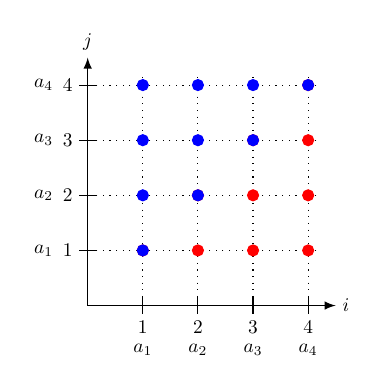
\begin{tikzpicture}[scale=0.7, transform shape]
        \tikzset{>=latex}

	\draw[->] (0,0) -- (4.5,0) node [right] {$i$};
	\draw[->] (0,0) -- (0,4.5) node [above] {$j$};
	\foreach \x in {1, 2, 3, 4} {
	    \draw [dotted] (\x,4.15) -- (\x,-0.15);
	    \draw [dotted] (4.15,\x) -- (-0.15,\x);
	    \draw  (\x,0.15) -- (\x,-0.15) node [below] {$\x$};
	    \draw  (0.15,\x) -- (-0.15,\x) node [left] {$\x$};
      \node (a) at (\x,-0.8) {$a_{\x}$};
      \node (b) at (-0.8,\x) {$a_{\x}$};
	    }
	\foreach \x in {1, 2, 3, 4} {
	    \foreach \y in {1,...,\x} {
        \filldraw [red] (\x,\y) circle (0.10);
		}
	    \foreach \y in {\x,...,4} {
        \filldraw [color=blue] (\x,\y) circle (0.10);
		}
	    }
        \end{tikzpicture}
    \end{center}
\end{center}
}
%-------------- end slide -------------------------------%}}}
%-------------- start slide -------------------------------%{{{ 31
\begin{frame}[fragile]
    \begin{proofnoend}
       We will prove this by induction. It is clear that when $n=2$,
       \begin{align*}
	   \det \begin{pmatrix} 1 & a_1 \cr 1 & a_2 \end{pmatrix}
	   = a_2-a_1
	   = \prod_{1\leq j<i\leq 2}(a_i-a_j).
       \end{align*}
       \bigskip

       \pause
       Assume that it is true for $n-1$.\pause~ Now let's consider the case $n$.
       Denote
	\begin{align*}
	    p(\textcolor{yellow}{x}) :=
	    \det\left[\begin{array}{ccccc}
        1                     & a_1                   & a_1^2                   & \cdots & a_1^{n-1}     \\
        1                     & a_2                   & a_2^2                   & \cdots & a_2^{n-1}     \\
        \vdots                & \vdots                & \vdots                  & \vdots & \vdots        \\
        1                     & a_{n-1}               & a_{n-1}^2               & \cdots & a_{n-1}^{n-1} \\
        \textcolor{yellow}{1} & \textcolor{yellow}{x} & \textcolor{yellow}{x^2} & \cdots & \textcolor{yellow}{x^{n-1}}
	    \end{array}\right].
	\end{align*}
    \end{proofnoend}

\end{frame}
%-------------- end slide -------------------------------%}}}
%-------------- start slide -------------------------------%{{{ 32
\begin{frame}[fragile]
    \begin{proofnoend}[continued]
	   Because $p(a_1) = \cdots = p(a_{n-1}) = 0$ (why?), $p(x)$ has to take the following form:
	       \begin{align*}
		   p(x) = c (x-a_1)(x-a_2) \cdots (x-a_{n-1}) .
	       \end{align*}
	       \vfill
	       \vspace{2em}
	   To identify the constant $c$, notice that $c$ is the coefficient for $x^{n-1}$.
	       By cofactor expansion of the determinant along the last row,
	       \begin{align*}
		   c &= (-1)^{n+n}
		    \det\left[\begin{array}{ccccc}
          1      & a_1     & a_1^2     & \cdots & a_1^{n-1}\\
          1      & a_2     & a_2^2     & \cdots & a_2^{n-1}\\
          \vdots & \vdots  & \vdots    & \vdots & \vdots \\
          1      & a_{n-1} & a_{n-1}^2 & \cdots & a_{n-1}^{n-1} \\
		    \end{array}\right]\\
		     &= \prod_{1\leq j<i\leq \alert{n-1}  }(a_i-a_j).
	       \end{align*}
    \end{proofnoend}
\end{frame}
%-------------- end slide -------------------------------%}}}
%-------------- start slide -------------------------------%{{{ 33
\begin{frame}[fragile]
\begin{proofnoend}[continued]
    Hence,
    \begin{align*}
      p(a_n) & = \textcolor{magenta}{\left( \prod_{1\leq j<i\leq \alert{n-1}  }(a_i-a_j)\right) }\times \textcolor{red}{(a_{n}-a_1)(a_{n}-a_2) \cdots (a_{n}-a_{n-1}) }
    \end{align*}
    \begin{center}
        \begin{center}
            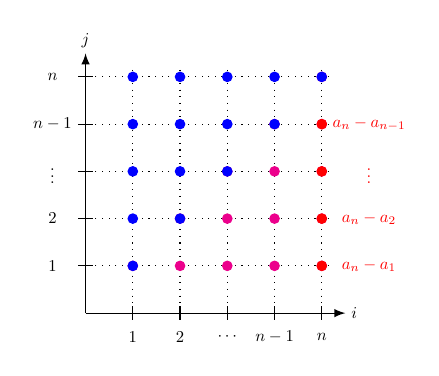
\begin{tikzpicture}[scale=0.6, transform shape]
            \tikzset{>=latex}

      \draw[->] (0,0) -- (5.5,0) node [right] {$i$};
      \draw[->] (0,0) -- (0,5.5) node [above] {$j$};
      \node at (1,-0.5) {$1$};
      \node at (2,-0.5) {$2$};
      \node at (3,-0.5) {$\cdots$};
      \node at (4,-0.5) {$n-1$};
      \node at (5,-0.5) {$n$};

      \node at (-0.7,1) {$1$};
      \node at (-0.7,2) {$2$};
      \node at (-0.7,3) {$\vdots$};
      \node at (-0.7,4) {$n-1$};
      \node at (-0.7,5) {$n$};

      \node[red] at (6,1) {$a_n-a_1$};
      \node[red] at (6,2) {$a_n-a_2$};
      \node[red] at (6,3) {$\vdots$};
      \node[red] at (6,4) {$a_n-a_{n-1}$};
      % \node at (6,5) {$n$};

      \foreach \x in {1, ..., 5} {
          \draw [dotted] (\x,5.15) -- (\x,-0.15);
          \draw [dotted] (5.15,\x) -- (-0.15,\x);
          \draw (\x,0.15) -- (\x,-0.15);
          \draw (0.15,\x) -- (-0.15,\x);
          }
      \foreach \x in {1, ..., 5} {
          \foreach \y in {1,...,\x} {
        \filldraw [magenta] (\x,\y) circle (0.10);
        }
          \foreach \y in {\x,...,5} {
        \filldraw [blue] (\x,\y) circle (0.1);
        }
          }
      \foreach \y in {1,...,4}{
          \filldraw [red] (5,\y) circle (0.10);
          }
            % \coordinate (L) at (3.1,0.4);
            % \coordinate (P0) at (0.2,1.6);
            % \coordinate (0) at (0,0);
            % \coordinate (P) at (3,2.22);
            % \draw ($(P)!-1cm!(P0)$)  -- (P) node [below]  {$P$} -- (P0) node [above] {$P_0$} -- ($(P0)!-1cm!(P)$) node [left] {$L$};
            % \draw [thick,->,color=blue] (P0) --coordinate [pos={1/2}] (m) node [above] {${\vec{d}}$} ($(P)!1cm!(P0)$);
            % \draw[dashed,->] (0) node [below] {$} -- (P0);
            % \draw[dashed,->] (0) -- (P);
            % \filldraw (P) circle (0.05);
            % \filldraw (P0) circle (0.05);
            % \filldraw (0) circle (0.05);
            \end{tikzpicture}
        \end{center}
    \end{center}
    \begin{align*}
        p(a_n) & =  \prod_{1\leq j<i\leq \alert{n}  }(a_i-a_j).
    \end{align*}
    \myQED
\end{proofnoend}
\end{frame}
%-------------- end slide -------------------------------%}}}
%-------------- start slide -------------------------------%{{{ 34
\frame{
\begin{example}
In our earlier example with the data points $(0,1)$, $(1,2)$, $(2,5)$ and $(3,10)$, we have
\[ a_1=0,\quad a_2=1,\quad a_3=2,\quad a_4=3\]
giving us the {\it Vandermonde} determinant
\[ \left|\begin{array}{rrrr}
    1 & 0 & 0 & 0 \\
    1 & 1 & 1 & 1 \\
    1 & 2 & 4 & 8 \\
    1 & 3 & 9 & 27
   \end{array}\right|
\]

\pause
According to the previous theorem, this determinant is equal to
\begin{align*}
      & (a_2-a_1) (a_3-a_1)(a_3-a_2)(a_4-a_1)(a_4-a_2)(a_4-a_3) \\
    = & (1-0)(2-0)(2-1)(3-0)(3-1)(3-2) \\
    = & 2\times 3\times 2      \\
    = & 12.
\end{align*}
\end{example}
}
%-------------- end slide -------------------------------%}}}
%-------------- start slide -------------------------------%{{{ 35
\frame{
\begin{corollary}
    The Vandermonde determinant is nonzero if $a_1, a_2, \ldots, a_n$ are distinct.
\end{corollary}
\vfill
\pause
\begin{emptytitle}
    This means that given $n$ data points
    $(x_1, y_1), (x_2,y_2),\ldots,(x_n,y_n)$ with
    \alert{distinct} $x_i$, then there is a
    unique interpolating polynomial
    \[ p(x)=r_0 + r_1x + r_2x^2 + \cdots + r_{n-1}x^{n-1}.\]
\end{emptytitle}
}
%-------------- end slide -------------------------------%}}}
\end{document}
